
\subsubsection{Глобальные модели реанализа погоды}
\label{sec:whether_models}

Разнородность архивных метеоданных и невозможность прямых измерений над океанами привела в 1980-х годах к необходимости реализации программ комплексного реанализа данных.

Европейский центр ECMWF начал программу реанализов с проекта FGGE (1979), затем последовали ERA-15 (1994) и ERA-40 (2001). 
Четвертое поколение ERA-Interim (2006–2019) стало де-факто стандартом для климатических исследований. 
ERA5, запущенный в 2017 году как оперативный сервис, представляет пятое поколение моделей и впервые обеспечил пространственно-временное разрешение (0.25°, 1 час) метеоданных накопленных с 1 января 1940 года~\cite{Hersbach2020ERA5}.

Альтернативой программе ERA5 является программа NASA MERRA (Modern-Era Retrospective analysis for Research and Applications), реализованная в 2008 году, охватывающий период с 1980 года. 
MERRA-2, запущенная в 2015 году, стала первым долговременным реанализом, ассимилирующим спутниковые наблюдения аэрозолей, позволяя вести учет радиационного воздействия пыли, морской соли, сульфатов и органических аэрозолей на климат, что важно для исследований радиационного баланса и качества воздуха.

Национальные центры NOAA начали серию реанализов с NCEP/NCAR Reanalysis (1996), охватывающего данные с 1948 года~\cite{saha2014ncep}. 
Climate Forecast System (CFS) был запущен в 2004 году, а его вторая версия CFSv2 -- в марте 2011 года. 
Обе эти системы ориентированы на связанное моделирование системы океан-атмосфера для долгосрочных сезонных прогнозов и климатических исследований.

В результате принципиальное различие между системами заключается в приоритетах ассимиляции. 
Технологически все они используют вариационную или ансамблевую ассимиляцию данных, но различаются базовыми моделями и схемами параметризации граничного слоя и конвекции воздуха. 
Для прикладных задач выбор реанализа определяется требуемыми переменными, так ERA5 предпочтителен для анализа ветровых параметров у поверхности, MERRA-2 -- для радиационного баланса и аэрозолей, CFSv2 -- для анализа долгосрочных климатических трендов.

Таким образом для задач оценки волновой экспозиции прибрежных территорий ERA5 представляет оптимальный выбор по нескольким причинам.
Во-первых, пространственное разрешение 0.25° и часовой шаг позволяют детально воспроизводить прибрежную циркуляцию, бризы и штормовые события.
Во-вторых, ERA5 включает параметры волнения океана (высота значительной волны, период, направление), рассчитанные интегрированной моделью WAM (WAve Model), что позволяет контролировать выполняемые расчеты. 
В-третьих, охват с 1940 года обеспечивает достаточную глубину временного ряда для климатологического анализа экстремумов и многолетних трендов. 
Наконец, открытый API Climate Data Store гарантирует оперативный программный доступ к данным без административных барьеров.

\subsubsection{Состав данных модели ERA5}

ERA5 представляет собой комплексный набор климатических данных, охватывающий более 240 переменных для атмосферы, поверхности суши и океана. 
Массив организован в четыре основные категории: 
\begin{itemize}
    \item приземные параметры (single levels);
    \item поля на уровнях давления (pressure levels); 
    \item ансамблевые оценки неопределенности;
    \item месячные осреднения~\cite{era5_single_levels_daily_earthdatahub}.
\end{itemize}

\begin{figure}
    \begin{center}
	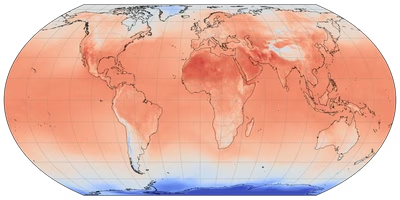
\includegraphics[width=100mm]{fig/part_2/ERA5.png}
	\caption{-- Пример визуализации глобальной карты распредеелния температур модели ERA5~\cite{era5_single_levels_daily_earthdatahub}}
	\label{pic:era5temp}
    \end{center}
\end{figure}


Приземный слой характеризуется набором переменных на стандартных высотах: температура воздуха и точка росы измеряются на высоте 2 метра (рисунок~\ref{pic:era5temp}), компоненты ветра -- на 10 и 100 метрах, также доступны порывы ветра и давление, приведенное к уровню моря. 
В верхних слоях атмосферы реанализ использует 137 модельных уровней от поверхности до высоты 80 км, на которых рассчитываются трехмерные поля температуры, влажности (удельной и относительной), всех компонент ветра, вертикальной скорости, геопотенциальной высоты, завихренности и дивергенции.

Радиационный баланс описывается потоками коротко- и длинноволнового излучения как на поверхности, так и на верхней границе атмосферы, дополненными УФ-радиацией, альбедо и условиями ясного неба. Осадки детализированы по шести типам: дождь, снег, мокрый снег, смешанные осадки, ледяной дождь и град.

Почвенные характеристики включают объемную влажность и температуру по четырем слоям глубиной 0–7, 7–28, 28–100 и 100–289 см (значения относятся к середине каждого слоя). 
Снежный покров представлен глубиной в водном эквиваленте, плотностью, температурой и скоростями таяния и накопления.

Для морской поверхности доступны температура, концентрация морского льда и параметр шероховатости Чарнока, определяющий обмен импульсом между атмосферой и океаном. 
Волнение детально описывается высотой значительной волны, средним периодом, направлением распространения, с разделением на ветровые волны и зыбь. 
Интеграция модели WAM в цикл ассимиляции обеспечивает физическую согласованность ветра и волн.

Помимо исходных переменных, ERA5 содержит производные климатические индексы: число дней с заморозками (минимальная температура ниже 0°C), тропических ночей с минимальной температурой выше 20°C, экстремумы температур и накопленные суммы осадков~\cite{era5_single_levels_daily_earthdatahub}.

Все данные доступны в стандартных форматах GRIB и NetCDF на регулярной сетке 0.25° для атмосферных параметров и 0.5° для волнения. 
Валидация на российских метеостанциях подтверждает высокую точность воспроизведения температурного режима с коэффициентами корреляции в пределах 0.8–0.95 и удовлетворительное воспроизведение динамики почвенной влаги и климатических характеристик~\cite{Titkova2023ERA5Land}.


\subsubsection{Механизм доступа и работы с данными ERA5}
\label{sec:whether_data}

Базовый механизм распространения данных ERA5 происходит через Climate Data Store (CDS) Copernicus~\cite{c3s_era5_single_levels_hourly}. 
Данные распространяются под лицензией Copernicus Products, разрешающей свободное использование, без территориальных ограничений, бессрочно и безвозмездно.
Однако для получения данных требуется регистрация личной учетной записи, после чего в личном профиле пользователя формируются UID (User ID) и персональный API Key, необходимые к включению в тело запроса.
Система предоставляет два способа получения данных: интерактивный веб-интерфейс и программный API.

Скачиваемые файлы организованы в две основные категории.
\begin{enumerate}
    \item Single-level data -- приземные, почвенные и океанские параметры.
    \item Pressure-level data -- атмосферные поля на изобарических уровнях (1000, 925, 850, 700, 500, 300, 250, 200~гПа и~др.).
\end{enumerate}


Обновление данных происходит ежедневно с задержкой примерно в 5 дней.
При этом данные за последние 3 месяца могут ретроспективно пересчитываться и замещаться финализированной версией.

Особенностью получения данных о ветере из CDS является то, что они формируются двумя ортогональными компанентами U и V.
U-компонента -- это зональная составляющая ветра на высоте 10 метров, горизонтальная скорость движения воздуха в направлении на восток, задаваемая в метрах в секунду (м/с). 
Положительные значения означают восточный ветер (движение воздуха с запада на восток), отрицательные -- западный ветер.
Аналогично V-компонента -- это меридианальная составляющая ветра на высоте 10 метров, то есть горизонтальная скорость движения воздуха в направлении на север. Положительные значения соответствуют северному ветру (с юга на север), отрицательные -- южному.

Совместно две компоненты полностью описывают вектор горизонтального ветра:
\begin{itemize}
    \item скорость ветра рассчитывается как: $\text{speed} = \sqrt{u^2 + v^2}$;
    \item направление ветра: $\text{direction} = \arctan2(u, v) \cdot \frac{180}{\pi} + 180°$.
\end{itemize}

Несмотря на кажущуюся неочевидность использование приведенных компонент удобнее для численных расчетов, так как оно непрерывно относительно перехода между румбами через 360°/0° и позволяет легче усреднять значения по модулям.

Кроме этого представляемый в результате формат организован в форме регулярной широтно-долготной сетки (regular latitude-longitude grid), что упрощает организацию запросов для больших площадных территорий.
Данные распространяются в форматах, стандартных для растровых климатических данных:
\begin{itemize}
    \item \texttt{GRIB} (GRIdded Binary) -- бинарный растровый формат метеорологических служб;
    \item \texttt{NetCDF} (Network Common Data Form) -- растровый формат для многомерных данных;
    \item \texttt{Zarr} -- облачно-оптимизированный растровый формат.
\end{itemize}

Для непосредственного получения и низкоуровневой работы с данным средствами python в работе используются следующие нестандартные модули:
\begin{itemize}
    \item \texttt{cdsapi} -- Climate Data Store API для загрузки данных с серверов Copernicus;
    \item \texttt{xarray} -- основной инструмент для работы с NetCDF и многомерными массивами;
    \item \texttt{netCDF4} -- библиотека для чтения формата NetCDF;
    \item \texttt{cfgrib} -- для чтения формата GRIB (альтернатива NetCDF).
\end{itemize}

Последующая обработка выполняется общеупотребимыми средствами python, такими как \texttt{numpy}, \texttt{geopandas} и \texttt{scipy}.

В рамках постобработки данных выполняется интерполяция данных для непосредственной точки расчета относительно исходной сетки данных, а также вычисление непосредственных параметров скорости и направления ветра.

Альтернативным источником получения метеоданных является бесплатный погодный API Open-Meteo, который агрегирует данные более 30 численных моделей погоды от национальных метеослужб (ECMWF, NOAA, DWD, Météo-France, JMA, UK Met Office и др.).
Сервис предоставляет унифицированный JSON API для доступа к прогнозам, историческим данным и реанализу ERA5 с 1940 года.

API работает через простые HTTP GET-запросы без необходимости регистрации, API-ключа или SDK для некоммерческого использования. 
Запрос принимает географические координаты и список переменных, возвращая почасовой временной ряд в формате JSON. 
Система автоматически выбирает модель с наивысшим пространственным разрешением для указанной точки. 
Данные нормализуются к часовому шагу независимо от исходного временного разрешения модели.

Таким образом, работа через этот сервис позволяет гарантировано получить в общем случае наиболее релевантные данные для конкретной точки.
Однако в случае выполнения запроса для множества точек рассматриваемый сервис не имеет средств кэширования и оптимизации запросов, вследствие чего возникает необходимость выполнения предварительных мини-запросов, опытным путем «испытывающих» локальную метео модель, соответствующую анализируемой области.

Для задач оценки волновой экспозиции Open-Meteo предоставляет морские прогнозы (высота волн, период, направление ветра) и доступ к архиву ERA5 через тот же API. 
Это упрощает механизмы работы с метеоданными в силу отсутствия  необходимости скачивания больших файлов NetCDF, использования специфичных пакетов для их обработки и получения персонального API ключа.
Таким образом, с учетом ограничения количества запросов на бесплатном тарифе Open-Meteo в 10 000 запросов/день этот сервис следует рассматривать как резервный в случае ограничения свободного доступа к прямому доступу к ERA5 через CDS API.

\subsubsection{Заключение}

В результате исторического развития метеорологии человечество пришло к качественно новому уровню «памяти о погоде» и пониманию оружающего мира. 
Реанализы вроде ERA5 воплощают эту память в виде непрерывного, физически согласованного описания атмосферы и океана, охватывающего десятилетия и континенты, тем самым замыкая цепочку от первых разрозненных наблюдений до глобальных цифровых архивов.  

Для прикладных задач, это означает, что исследователь больше не ограничен ни национальными границами наблюдательных сетей, ни ведомственными барьерами доступа к данным.
Достаточно один раз настроить доступ к Climate Data Store, чтобы опираться на единый, воспроизводимый источник метеоинформации с высоким пространственно-временным разрешением, надеясь, что политическапя турбулетность оружающего мира не разрушит хрупкий баланс до сих пор сохраняющийся в научном обществе. 
При этом агрегаторы вроде Open-Meteo становятся удобным запасной точкой доступа к этой инфраструктуре -- позволяя быстро получать точечные временные ряды без работы с тяжелыми NetCDF/GRIB файлами и сложными API, дополняя прямой доступ к ERA5. 
В совокупности это создает для современного инженера и исследователя набор уникальных возможностей, когда у него есть практически неограниченный по объему и детализации архив метеоданных, к которому можно обращаться программно и автоматически, интегрируя климатическую «память» планеты напрямую в расчетные модели и системы поддержки принятия решений.  
